\label{tecfile:TecplotUseage}
\section*{Step~\ref{step:Tecplot1}: Run \tecplot\ to Examine the Built Project}
You can run \tecplot\ and load the \tecplot\ layout file \_\verb+build.lay+ by typing:
\begin{verbatim}
    tec360 _build.lay
\end{verbatim}
Some key features to note are:
\begin{itemize}
    \item A \tecplot\ window should open: \\ \\
        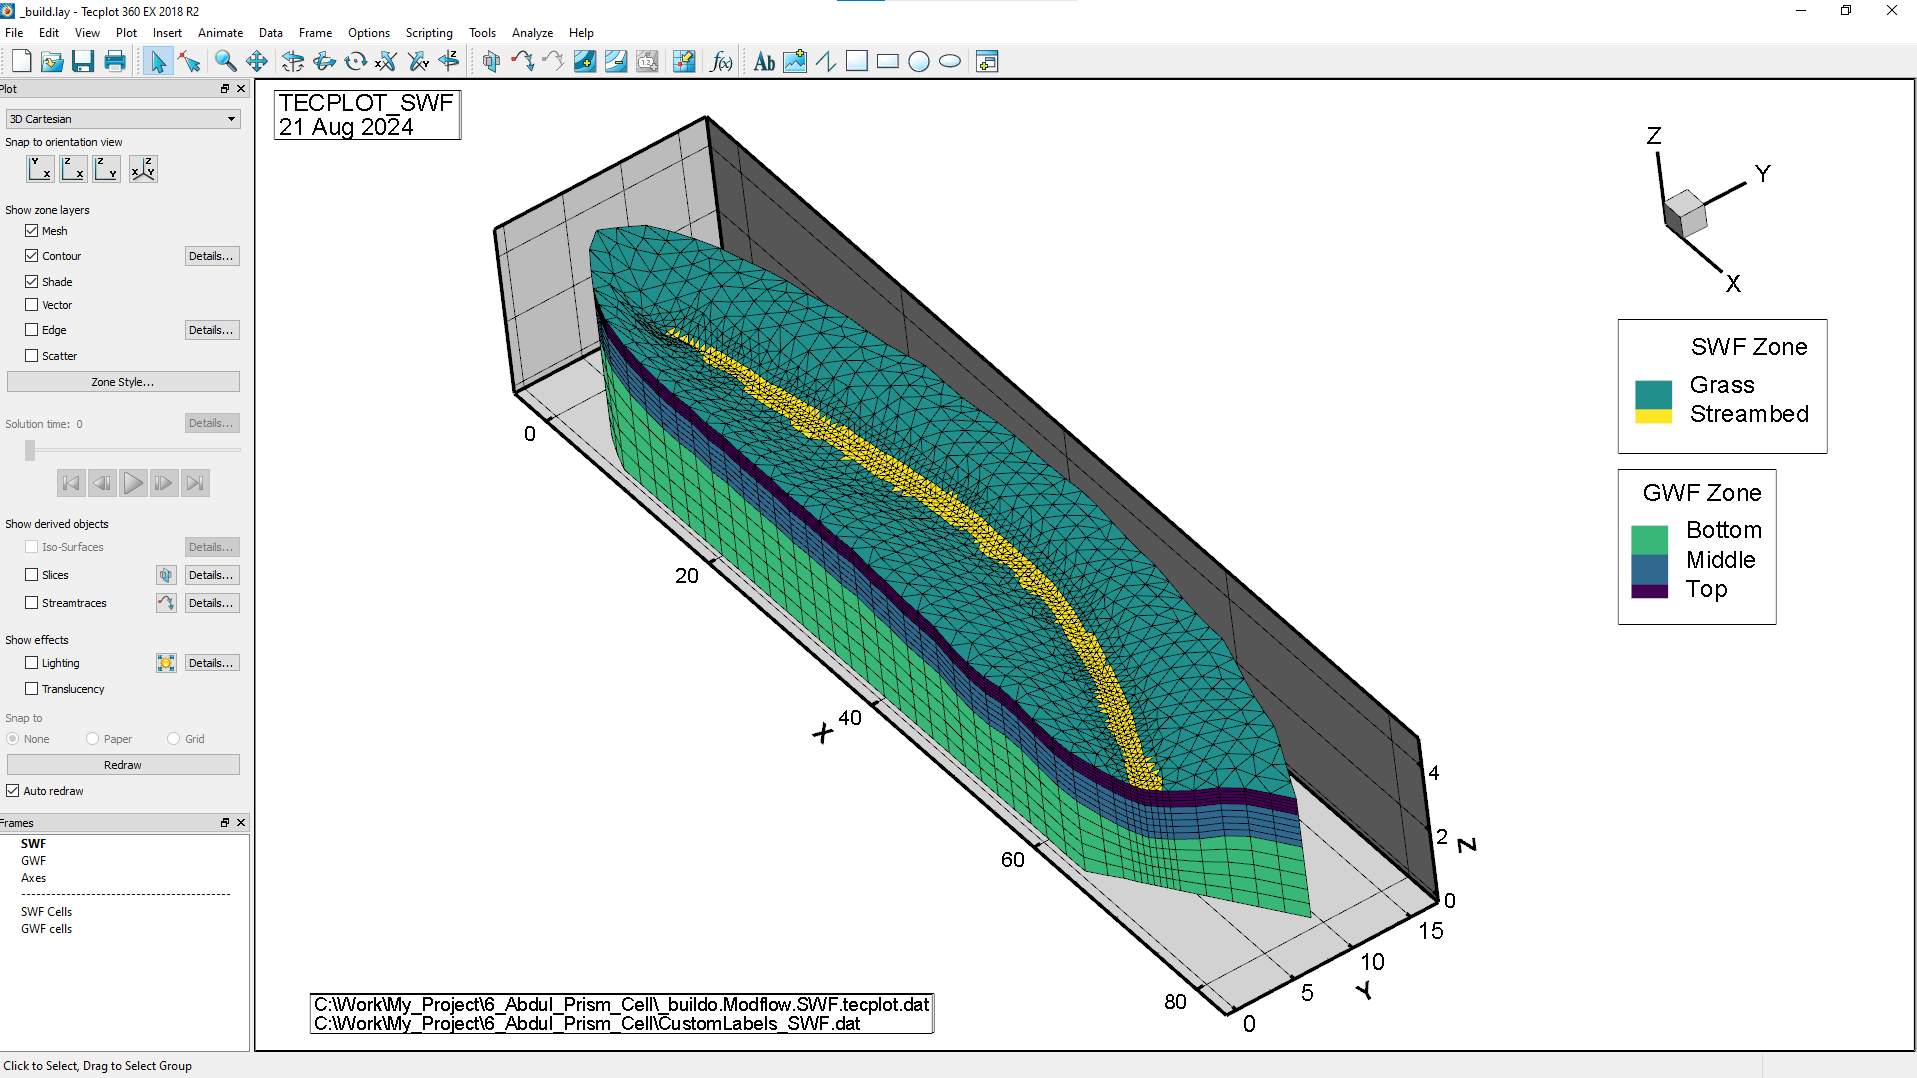
\includegraphics[width=0.8\textwidth]{TecplotBuild} \\ \\
    This \tecplot\ layout file has been constructed with multiple frames (see lower left 'Frames' window) showing details about the\swf\ and\gwf\ model domains. This default view shows the distribution of the various materials defined in the model, such as the\swf\ domain materials called 'Grass' and 'Streambed'.  Detailed information about manipulating the data in \tecplot\ to produce the desired plots is discussed in Section~\ref{Tecplot}.
    \item \tecplot\ data can be probed using the probe tool 
\includegraphics{ProbeToolButton} .  Here we see the results of probing a location in the\swf\ domain: \\
        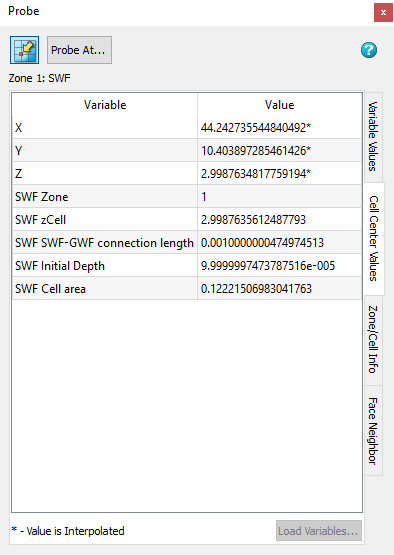
\includegraphics[width=0.4\textwidth]{SWFprobe} \\
       \swf\ results were returned because the\swf\ frame is at the front of the frame stack.
    \item In order to probe the\gwf\ domain we have to move it to the front of the stack: \\
            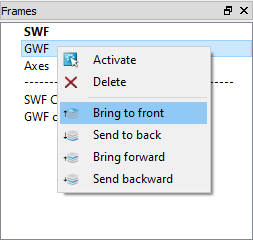
\includegraphics[width=0.4\textwidth]{BringToFront} \\
          Here we see the results of probing a location in the\gwf\ domain: \\
            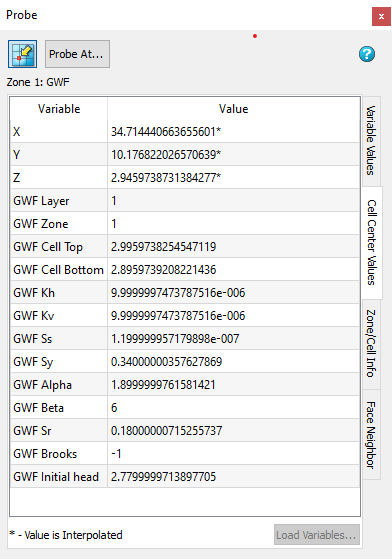
\includegraphics[width=0.4\textwidth]{GWFprobe} \\

\end{itemize}

